\documentclass[tikz,border=8pt]{standalone}
\usepackage{amsmath,amssymb}
\usetikzlibrary{arrows.meta,automata,positioning,quotes}
\begin{document}
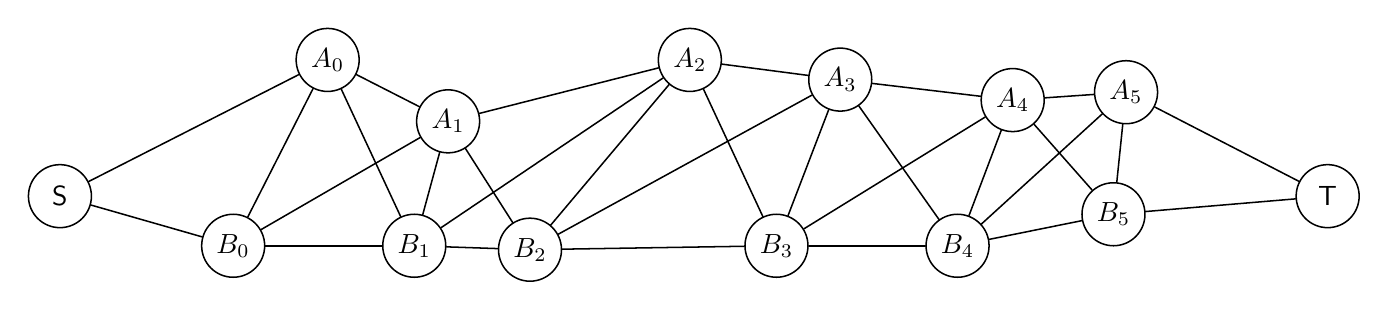
\begin{tikzpicture}[x=1cm,y=1cm]
\tikzset{
  graphnode/.style={circle,draw=black,line width=0.55pt,minimum size=8mm,inner sep=1pt,font=\sffamily},
  graphedge/.style={draw=black,line width=0.55pt,line cap=round,line join=round},
  directed/.style={graphedge,-{Stealth[length=2.4mm,width=2.0mm]}},
  undirected/.style={graphedge}
}
\node[graphnode] (n_A0) at (0.35,1.73) {$A_{0}$};
\node[graphnode] (n_A1) at (1.88,0.95) {$A_{1}$};
\node[graphnode] (n_A2) at (4.95,1.73) {$A_{2}$};
\node[graphnode] (n_A3) at (6.86,1.48) {$A_{3}$};
\node[graphnode] (n_A4) at (9.05,1.22) {$A_{4}$};
\node[graphnode] (n_A5) at (10.49,1.32) {$A_{5}$};
\node[graphnode] (n_B0) at (-0.85,-0.63) {$B_{0}$};
\node[graphnode] (n_B1) at (1.45,-0.63) {$B_{1}$};
\node[graphnode] (n_B2) at (2.92,-0.68) {$B_{2}$};
\node[graphnode] (n_B3) at (6.05,-0.63) {$B_{3}$};
\node[graphnode] (n_B4) at (8.35,-0.63) {$B_{4}$};
\node[graphnode] (n_B5) at (10.33,-0.23) {$B_{5}$};
\node[graphnode] (n_S) at (-3.05,0.00) {S};
\node[graphnode] (n_T) at (13.05,0.00) {T};
\draw[undirected] (n_A0) -- (n_A1);
\draw[undirected] (n_A1) -- (n_A2);
\draw[undirected] (n_A2) -- (n_A3);
\draw[undirected] (n_A3) -- (n_A4);
\draw[undirected] (n_A4) -- (n_A5);
\draw[undirected] (n_B0) -- (n_B1);
\draw[undirected] (n_B1) -- (n_B2);
\draw[undirected] (n_B2) -- (n_B3);
\draw[undirected] (n_B3) -- (n_B4);
\draw[undirected] (n_B4) -- (n_B5);
\draw[undirected] (n_A0) -- (n_B0);
\draw[undirected] (n_A1) -- (n_B1);
\draw[undirected] (n_A2) -- (n_B2);
\draw[undirected] (n_A3) -- (n_B3);
\draw[undirected] (n_A4) -- (n_B4);
\draw[undirected] (n_A5) -- (n_B5);
\draw[undirected] (n_A0) -- (n_B1);
\draw[undirected] (n_B1) -- (n_A2);
\draw[undirected] (n_A2) -- (n_B3);
\draw[undirected] (n_B3) -- (n_A4);
\draw[undirected] (n_A4) -- (n_B5);
\draw[undirected] (n_B0) -- (n_A1);
\draw[undirected] (n_A1) -- (n_B2);
\draw[undirected] (n_B2) -- (n_A3);
\draw[undirected] (n_A3) -- (n_B4);
\draw[undirected] (n_B4) -- (n_A5);
\draw[undirected] (n_S) -- (n_A0);
\draw[undirected] (n_S) -- (n_B0);
\draw[undirected] (n_T) -- (n_A5);
\draw[undirected] (n_T) -- (n_B5);
\end{tikzpicture}
\end{document}
